% begin module algebraic-functions
\begin{frame}
\frametitle{Algebraic Functions}
\begin{definition}[Algebraic Function]
A function in $x$ that can be constructed using $x$, constants, and finitely many of the operations $+, -, *, /,$ and $\sqrt[n]{~}$ is called an algebraic function.

\uncover<2->{{\footnotesize Outside of Calculus I: function $f(x)$ = algebraic if it satisfies a polynomial equation with polynomial coefficients, i.e., $a_0(x) +a_1(x)f(x)+\dots +a_n(x) \left(f(x)\right)^n=0$ for some polynomials  $a_i(x)$.}}
\end{definition}
\uncover<3->{
Examples.
\begin{tabular}{ccc}
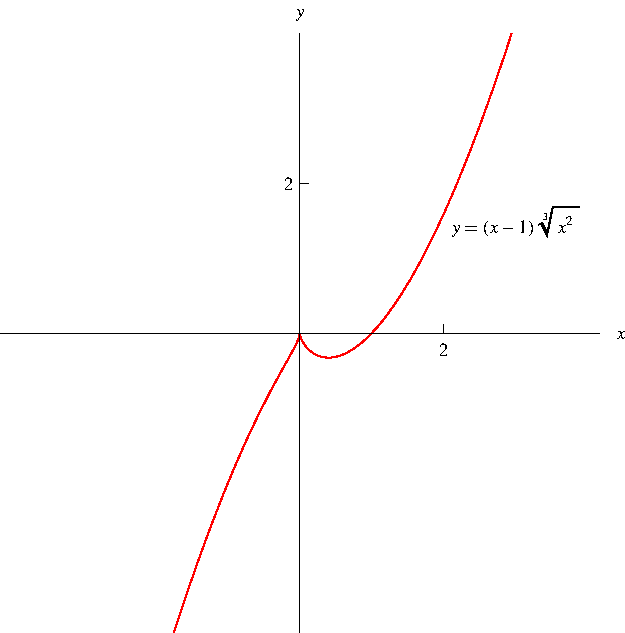
\includegraphics[height=3.8cm]{precalculus/pictures/01-02-algebraic1.pdf}&%
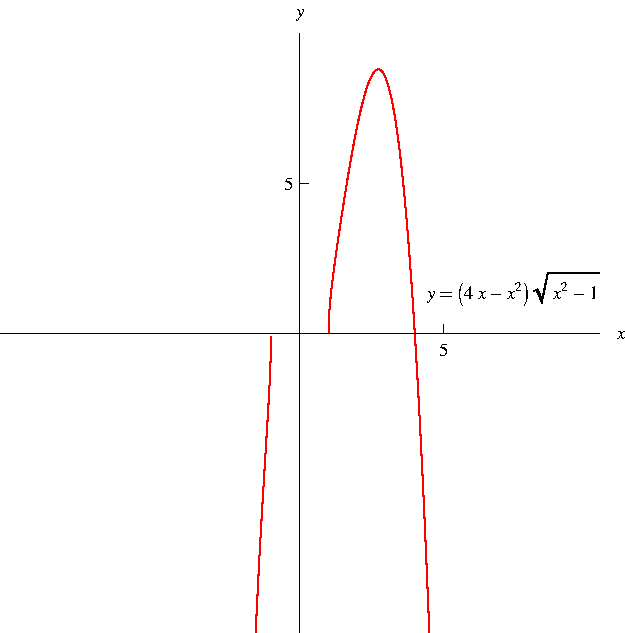
\includegraphics[height=3.8cm]{precalculus/pictures/01-02-algebraic2.pdf}&%
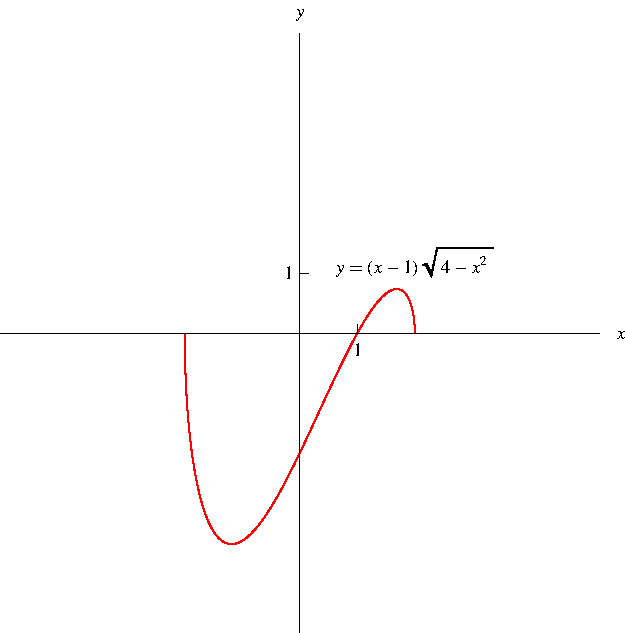
\includegraphics[height=3.8cm]{precalculus/pictures/01-02-algebraic3.pdf}%
\end{tabular}
}
\end{frame}
% end module algebraic-functions
